\chapter*{}                         % Заголовок
\addcontentsline{toc}{chapter}{Введение}    % Добавляем его в оглавление

\newcommand{\actuality}{}
\newcommand{\progress}{}
\newcommand{\aim}{{\textbf\aimTXT}}
\newcommand{\tasks}{\textbf{\tasksTXT}}
\newcommand{\novelty}{\textbf{\noveltyTXT}}
\newcommand{\influence}{\textbf{\influenceTXT}}
\newcommand{\methods}{\textbf{\methodsTXT}}
\newcommand{\defpositions}{\textbf{\defpositionsTXT}}
\newcommand{\reliability}{\textbf{\reliabilityTXT}}
\newcommand{\probation}{\textbf{\probationTXT}}
\newcommand{\contribution}{\textbf{\contributionTXT}}
\newcommand{\publications}{\textbf{\publicationsTXT}}

{\fontsize{14pt}{14.9pt}\selectfont
Сертификация -- процесс подтверждения соответствия характеристик товара определенным стандартам.

Сертификация не является универсальным способом 
решения всех существующих проблем в 
области информационной безопасности, однако 
сегодня это единственный реально функционирующий 
механизм, который обеспечивает независимый 
контроль качества средств защиты информации.
При грамотном применении механизм сертификации 
позволяет достаточно успешно решать задачу 
достижения гарантированного уровня защищенности автоматизированных систем.

{\actuality} Отсутствие недекларированных возможностей в скомпилированном
объектном файле является ключевым аспектом сертификации ПО.
Сертификация программного обеспечения необходима для 
подтверждения требований заказчика к защите 
информации, к выполнению функциональных 
и технических задач и к обеспечению работы ПО в целом.

\begin{figure}[!htbp]
    \centerfloat{
        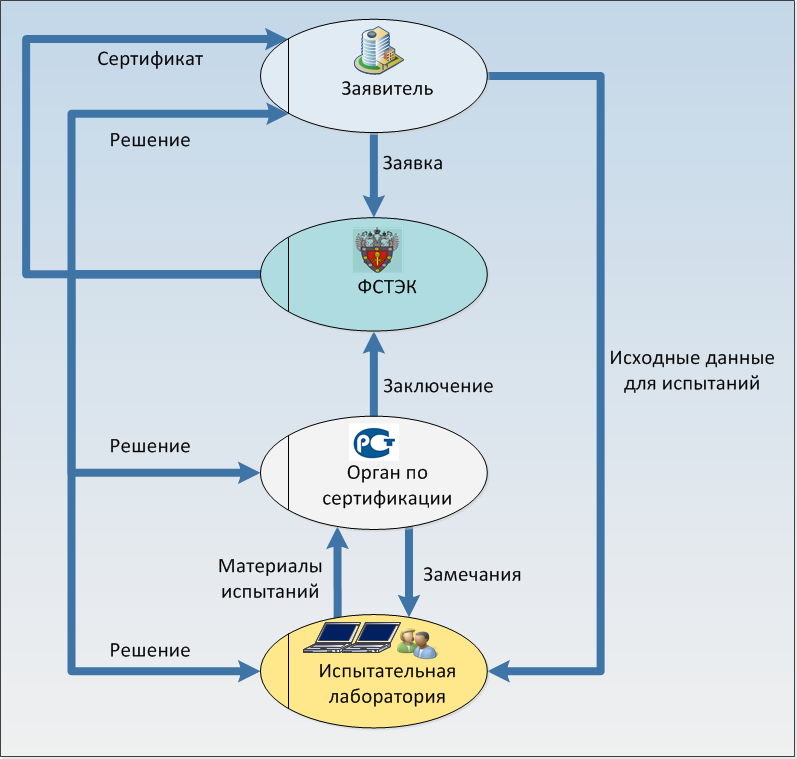
\includegraphics[width=\linewidth]{images/certification.png}
    }
    \caption{Процесс сертификации программного обеспечения во ФСТЭК\label{fig:fstak-cert}}
\end{figure}

Но существуют опасения, возникающие не на пустом месте,
что на любом из этапов сборки программы из
исходных кодов, в ней может появиться программная 
закладка \autocite{compile-a-virus, ken-thompson-hack}

Чтобы подобные ситуации исключить, применяется техника статического 
анализа исходных кодов, динамического анализа -- анализа пройденных 
программой трасс и последующее сравнение результатов обоих анализов.

На данный момент не существует открытых программных решений,
позволяющих проводить сертификацию программного обеспечения в описанном ранее формате.
Самое близкое по назначению ПО это статические анализаторы \autocite{c-static-analysis},
и так использующиеся как составная часть в процессе сертификации.
Помимо них существует свободное программное обеспечение от корпорации Microsoft --
Microsoft Application Inspector \autocite{microsoft-application-inspector}, но оно
взаимодействует только с исходными кодами программы, распознавая паттерны и назначение
функций.
Помимо свободных программ существует утилита анализа ядра Linux от ООО Фирма <<Анкад>>. 
В ней проводится статический, динамический и сравнительные анализы, но программа не умеет
работать с чем либо, кроме ядра Linux и сертифицировать что-либо еще с помощью нее не получится.
ООО Фирма <<Анкад>> на \autoref{fig:fstak-cert} выступает испытательной лабораторией.

\begin{figure}[!htbp]
    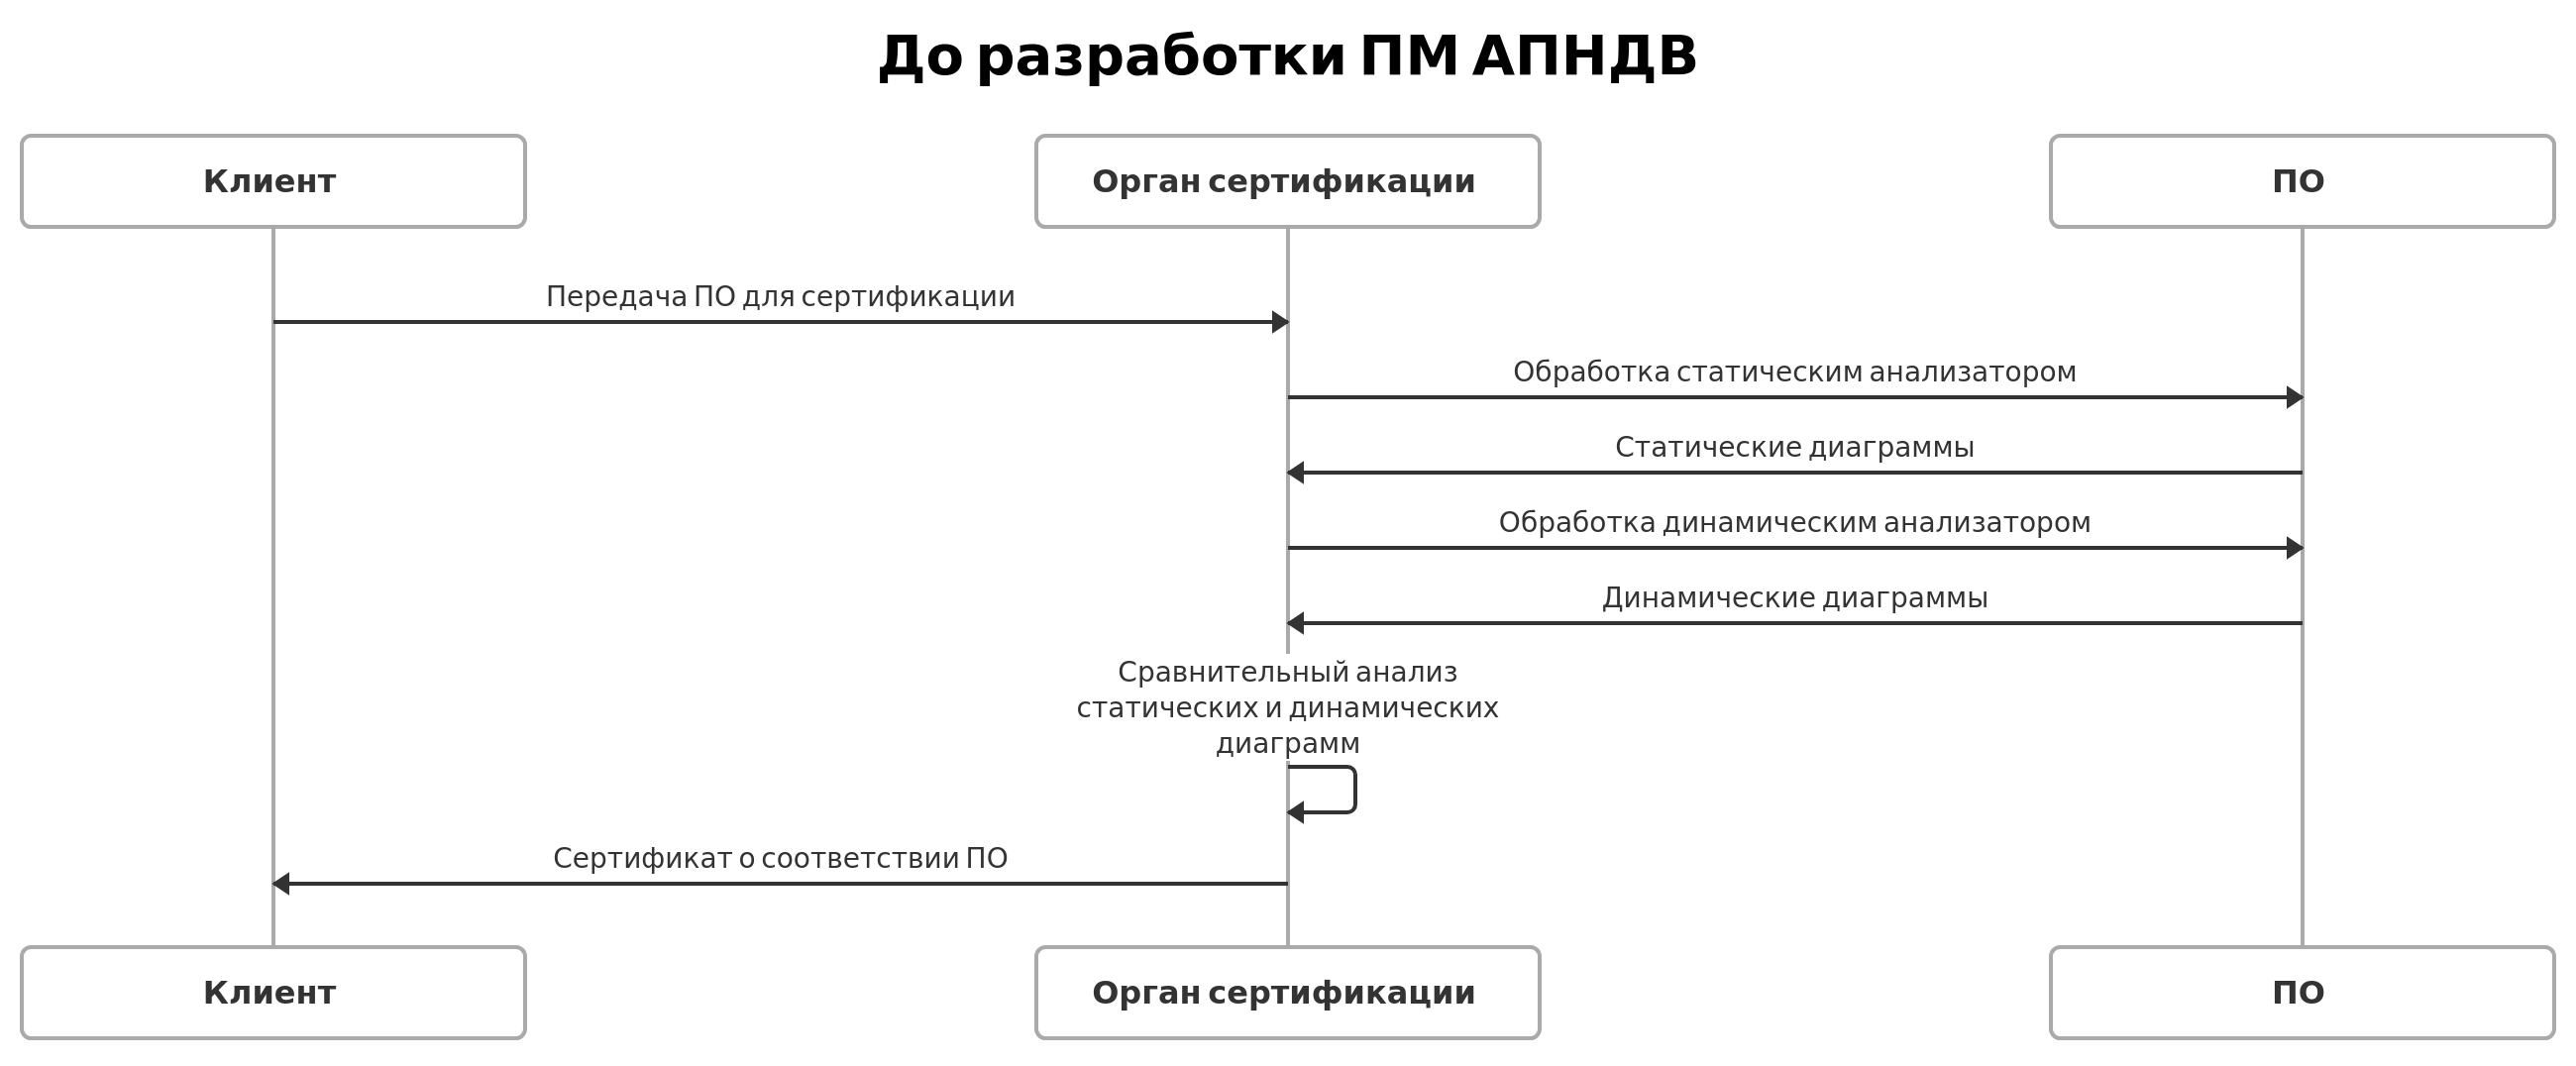
\includegraphics[width=\textwidth,height=\textheight,keepaspectratio]{images/uml_before_cropped.png}
    \caption{Процесс проведения сертификации раньше\label{fig:how-cert-was-before}}
\end{figure}

Получается, что на рынке невозможно найти комбинированных решений, 
с помощью которых было бы возможно провести процесс сертификации любого ПО. 
Для каждого конкретного проекта приходится использовать различные статические анализаторы, 
динамические анализаторы, что приводит к дублированию, по своей сути, кода и выполняемых действий, которые нужны для сертификации ПО.
Это ведет к разрастанию кодовой базы компании и нарастающим трудностям в последующей поддержке
каждого отдельного решения, что в свою очередь ведет к увеличению затрат компании.

Чтобы унифицировать разрабатываемое ПО для сертификации, было решено разбить {\ProgModule}
на модули, разделенные по ответственности и не знающие друг о друге. Это обеспечивает
удобство в редактировании, замене и изменении модулей, а при сохранении формата выдаваемой информации
 -- инкапсуляцию изменений только на конкретном модуле.

Так как модули не знают друг о друге, то и работают они в условиях ограниченной информации.
Модуль статического анализа обрабатывает только исходные коды, выдавая список статических
вызовов. Модуль динамического анализа работает с программой без отладочных символов,
собирая информацию на уровне машинных инструкций.

Данный подход помогает приблизить процесс сертификации к <<боевым>> условиям.

\ifsynopsis
Этот абзац появляется только в~автореферате.
Для формирования блоков, которые будут обрабатываться только в~автореферате,
заведена проверка условия \verb!\!\verb!ifsynopsis!.
Значение условия задаётся в~основном файле документа (\verb!synopsis.tex! для
автореферата).
\else
% Этот абзац появляется только в~диссертации.
% Через проверку условия \verb!\!\verb!ifsynopsis!, задаваемого в~основном файле
% документа (\verb!dissertation.tex! для диссертации), можно сделать новую
% команду, обеспечивающую появление цитаты в~диссертации, но~не~в~автореферате.
\fi

% {\progress}
% Этот раздел должен быть отдельным структурным элементом по
% ГОСТ, но он, как правило, включается в описание актуальности
% темы. Нужен он отдельным структурынм элемементом или нет ---
% смотрите другие диссертации вашего совета, скорее всего не нужен.

{\aim} данной работы является ускорение проведения процесса сертификации
программ написанных на языках программирования C/C++.

Для~достижения поставленной цели необходимо решить следующие {\tasks}:
\begin{enumerate}[label={\arabic*)}]
  \item анализ текущих программных решений для проведения 
        статического и динамического анализа, 
        выбор наиболее подходящего в плане универсальности 
        и расширяемости;
  \item анализ языков программирования для выбора наиболее производительного,
        надежного и легкоподдерживаемого;
  \item разработка алгоритма работы программы;
  \item разработка структур данных;
  \item разбиение функционала {\ProgModule} на модули по ответственности;
  \item разработка алгоритма передачи данных между модулями.
\end{enumerate}


% {\novelty}
% \begin{enumerate}
%   \item Впервые \ldots
%   \item Впервые \ldots
%   \item Было выполнено оригинальное исследование \ldots
% \end{enumerate}

{\influence} проекта состоит в унификации процесса сертификации ПО на отсутствие НДВ.

\begin{figure}[!htbp]
    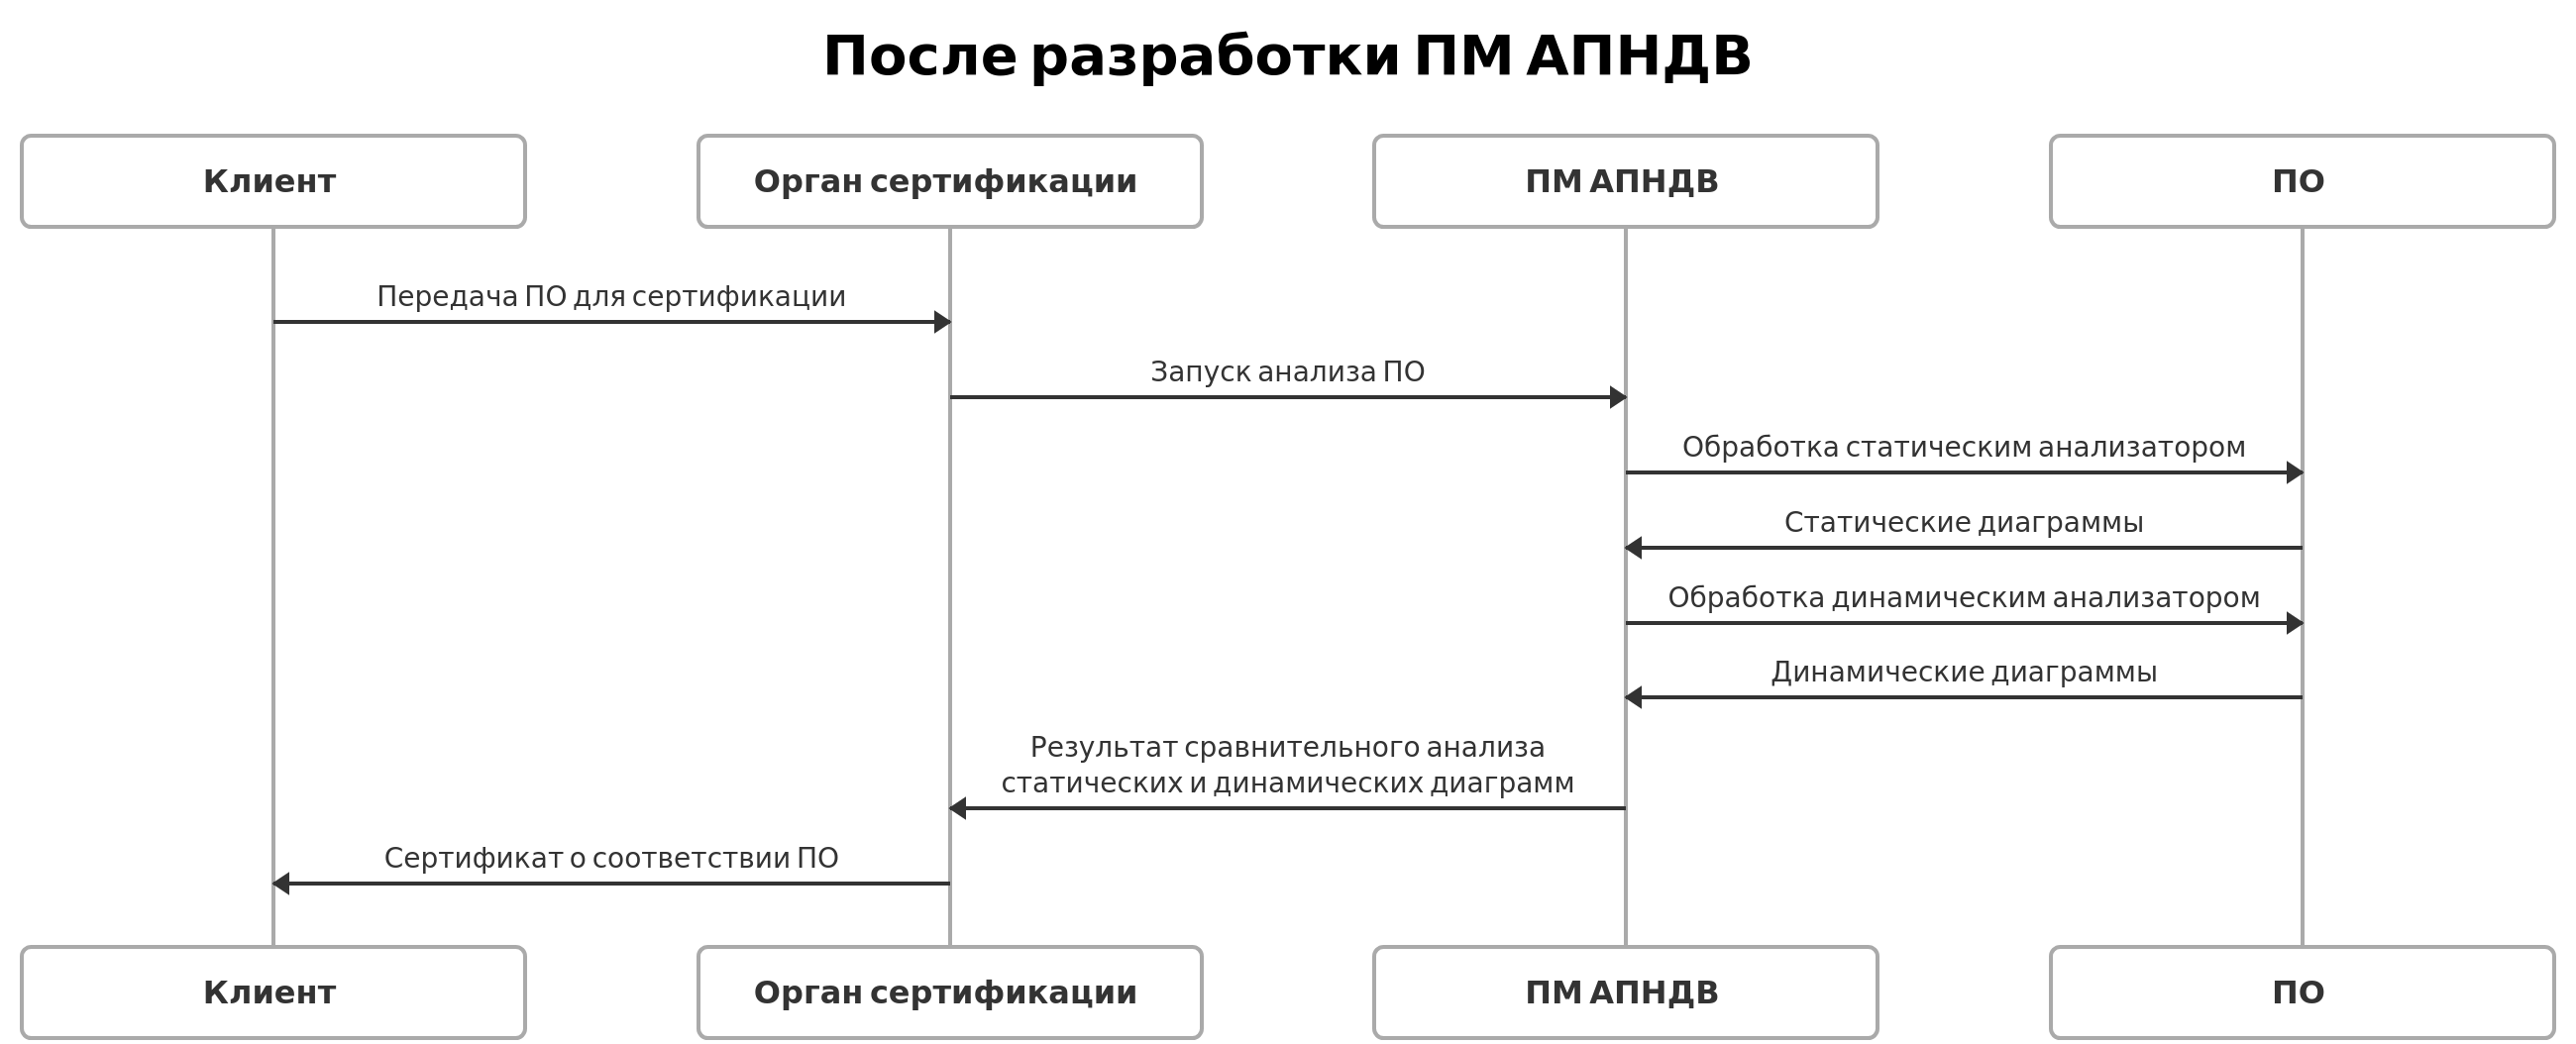
\includegraphics[width=\textwidth,height=\textheight,keepaspectratio]{images/uml_after_cropped.png}
    \caption{Процесс проведения сертификации сейчас\label{fig:how-cert-is-now}}
\end{figure}

%{\methods} \ldots

%{\defpositions}
%\begin{enumerate}
%  \item Первое положение
%\end{enumerate}
%В папке Documents можно ознакомиться в решением совета из Томского ГУ
%в~файле \verb+Def_positions.pdf+, где обоснованно даются рекомендации
%по~формулировкам защищаемых положений.

% {\reliability} полученных результатов обеспечивается \ldots \ Результаты находятся в соответствии с результатами, полученными другими авторами.
% 
% 
% {\probation}
% Основные результаты работы докладывались~на:
% перечисление основных конференций, симпозиумов и~т.\:п.
% 
% {\contribution} Автор принимал активное участие \ldots
% 
% \ifnumequal{\value{bibliosel}}{0}
% {%%% Встроенная реализация с загрузкой файла через движок bibtex8. (При желании, внутри можно использовать обычные ссылки, наподобие `\cite{vakbib1,vakbib2}`).
%     {\publications} Основные результаты по теме диссертации изложены в XX печатных изданиях,
%     X из которых изданы в журналах, рекомендованных ВАК,
%     X "--- в тезисах докладов.
% }%
% {%%% Реализация пакетом biblatex через движок biber
%     \begin{refsection}[bl-author]
%         % Это refsection=1.
%         % Процитированные здесь работы:
%         %  * подсчитываются, для автоматического составления фразы "Основные результаты ..."
%         %  * попадают в авторскую библиографию, при usefootcite==0 и стиле `\insertbiblioauthor` или `\insertbiblioauthorgrouped`
%         %  * нумеруются там в зависимости от порядка команд `\printbibliography` в этом разделе.
%         %  * при использовании `\insertbiblioauthorgrouped`, порядок команд `\printbibliography` в нём должен быть тем же (см. biblio/biblatex.tex)
%         %
%         % Невидимый библиографический список для подсчёта количества публикаций:
%         \printbibliography[heading=nobibheading, section=1, env=countauthorvak,          keyword=biblioauthorvak]%
%         \printbibliography[heading=nobibheading, section=1, env=countauthorwos,          keyword=biblioauthorwos]%
%         \printbibliography[heading=nobibheading, section=1, env=countauthorscopus,       keyword=biblioauthorscopus]%
%         \printbibliography[heading=nobibheading, section=1, env=countauthorconf,         keyword=biblioauthorconf]%
%         \printbibliography[heading=nobibheading, section=1, env=countauthorother,        keyword=biblioauthorother]%
%         \printbibliography[heading=nobibheading, section=1, env=countauthor,             keyword=biblioauthor]%
%         \printbibliography[heading=nobibheading, section=1, env=countauthorvakscopuswos, filter=vakscopuswos]%
%         \printbibliography[heading=nobibheading, section=1, env=countauthorscopuswos,    filter=scopuswos]%
%         %
%         \nocite{*}%
%         %
%         {\publications} Основные результаты по теме диссертации изложены в~\arabic{citeauthor}~печатных изданиях,
%         \arabic{citeauthorvak} из которых изданы в журналах, рекомендованных ВАК\sloppy%
%         \ifnum \value{citeauthorscopuswos}>0%
%             , \arabic{citeauthorscopuswos} "--- в~периодических научных журналах, индексируемых Web of~Science и Scopus\sloppy%
%         \fi%
%         \ifnum \value{citeauthorconf}>0%
%             , \arabic{citeauthorconf} "--- в~тезисах докладов.
%         \else%
%             .
%         \fi
%     \end{refsection}%
%     \begin{refsection}[bl-author]
%         % Это refsection=2.
%         % Процитированные здесь работы:
%         %  * попадают в авторскую библиографию, при usefootcite==0 и стиле `\insertbiblioauthorimportant`.
%         %  * ни на что не влияют в противном случае
%         \nocite{vakbib2}%vak
%         \nocite{bib1}%other
%         \nocite{confbib1}%conf
%     \end{refsection}%
%         %
%         % Всё, что вне этих двух refsection, это refsection=0,
%         %  * для диссертации - это нормальные ссылки, попадающие в обычную библиографию
%         %  * для автореферата:
%         %     * при usefootcite==0, ссылка корректно сработает только для источника из `external.bib`. Для своих работ --- напечатает "[0]" (и даже Warning не вылезет).
%         %     * при usefootcite==1, ссылка сработает нормально. В авторской библиографии будут только процитированные в refsection=0 работы.
%         %
%         % Невидимый библиографический список для подсчёта количества внешних публикаций
%         % Используется, чтобы убрать приставку "А" у работ автора, если в автореферате нет
%         % цитирований внешних источников.
%         % Замедляет компиляцию
%     \ifsynopsis
%     \ifnumequal{\value{draft}}{0}{
%       \printbibliography[heading=nobibheading, section=0, env=countexternal,          keyword=biblioexternal]%
%     }{}
%     \fi
% }
% 
% При использовании пакета \verb!biblatex! будут подсчитаны все работы, добавленные
% в файл \verb!biblio/author.bib!. Для правильного подсчёта работ в~различных
% системах цитирования требуется использовать поля:
% \begin{itemize}
%         \item \texttt{authorvak} если публикация индексирована ВАК,
%         \item \texttt{authorscopus} если публикация индексирована Scopus,
%         \item \texttt{authorwos} если публикация индексирована Web of Science,
%         \item \texttt{authorconf} для докладов конференций,
%         \item \texttt{authorother} для других публикаций.
% \end{itemize}
% Для подсчёта используются счётчики:
% \begin{itemize}
%         \item \texttt{citeauthorvak} для работ, индексируемых ВАК,
%         \item \texttt{citeauthorscopus} для работ, индексируемых Scopus,
%         \item \texttt{citeauthorwos} для работ, индексируемых Web of Science,
%         \item \texttt{citeauthorvakscopuswos} для работ, индексируемых одной из трёх баз,
%         \item \texttt{citeauthorscopuswos} для работ, индексируемых Scopus или Web of~Science,
%         \item \texttt{citeauthorconf} для докладов на конференциях,
%         \item \texttt{citeauthorother} для остальных работ,
%         \item \texttt{citeauthor} для суммарного количества работ.
% \end{itemize}
% % Счётчик \texttt{citeexternal} используется для подсчёта процитированных публикаций.
% 
% Для добавления в список публикаций автора работ, которые не были процитированы в
% автореферате требуется их~перечислить с использованием команды \verb!\nocite! в
% \verb!Synopsis/content.tex!.
 % Характеристика работы по структуре во введении и в автореферате не отличается (ГОСТ Р 7.0.11, пункты 5.3.1 и 9.2.1), потому её загружаем из одного и того же внешнего файла, предварительно задав форму выделения некоторым параметрам

\textbf{Объем и структура работы:}

Диссертация состоит из~введения, трёх глав,
заключения и~двух приложений.
% на случай ошибок оставляю исходный кусок на месте, закомментированным
Полный объём диссертации составляет  \ref*{TotPages}~страницу
с~\totalfigures{}~рисунками и~\totaltables{}~таблицами. Список литературы
содержит \total{citenum}~наименований.

}
